%%%% APÊNDICE B
%%
%% Texto ou documento elaborado pelo autor, a fim de complementar sua argumentação, sem prejuízo da unidade nuclear do trabalho.

%% Título e rótulo de apêndice (rótulos não devem conter caracteres especiais, acentuados ou cedilha)
\chapter{Prototype Photos}\label{app:photos}

\begin{figure}[H]
	\centering
	\caption[Frontal view of the prototype]{Frontal view of the prototype}
	\includegraphics[width=0.8\textwidth]{./images/20221204_164252.jpg}
    \fonte{}
\end{figure}

\begin{figure}[H]
	\centering
	\caption[Top view displaying the products in the cart]{Top view displaying the products in the cart}
    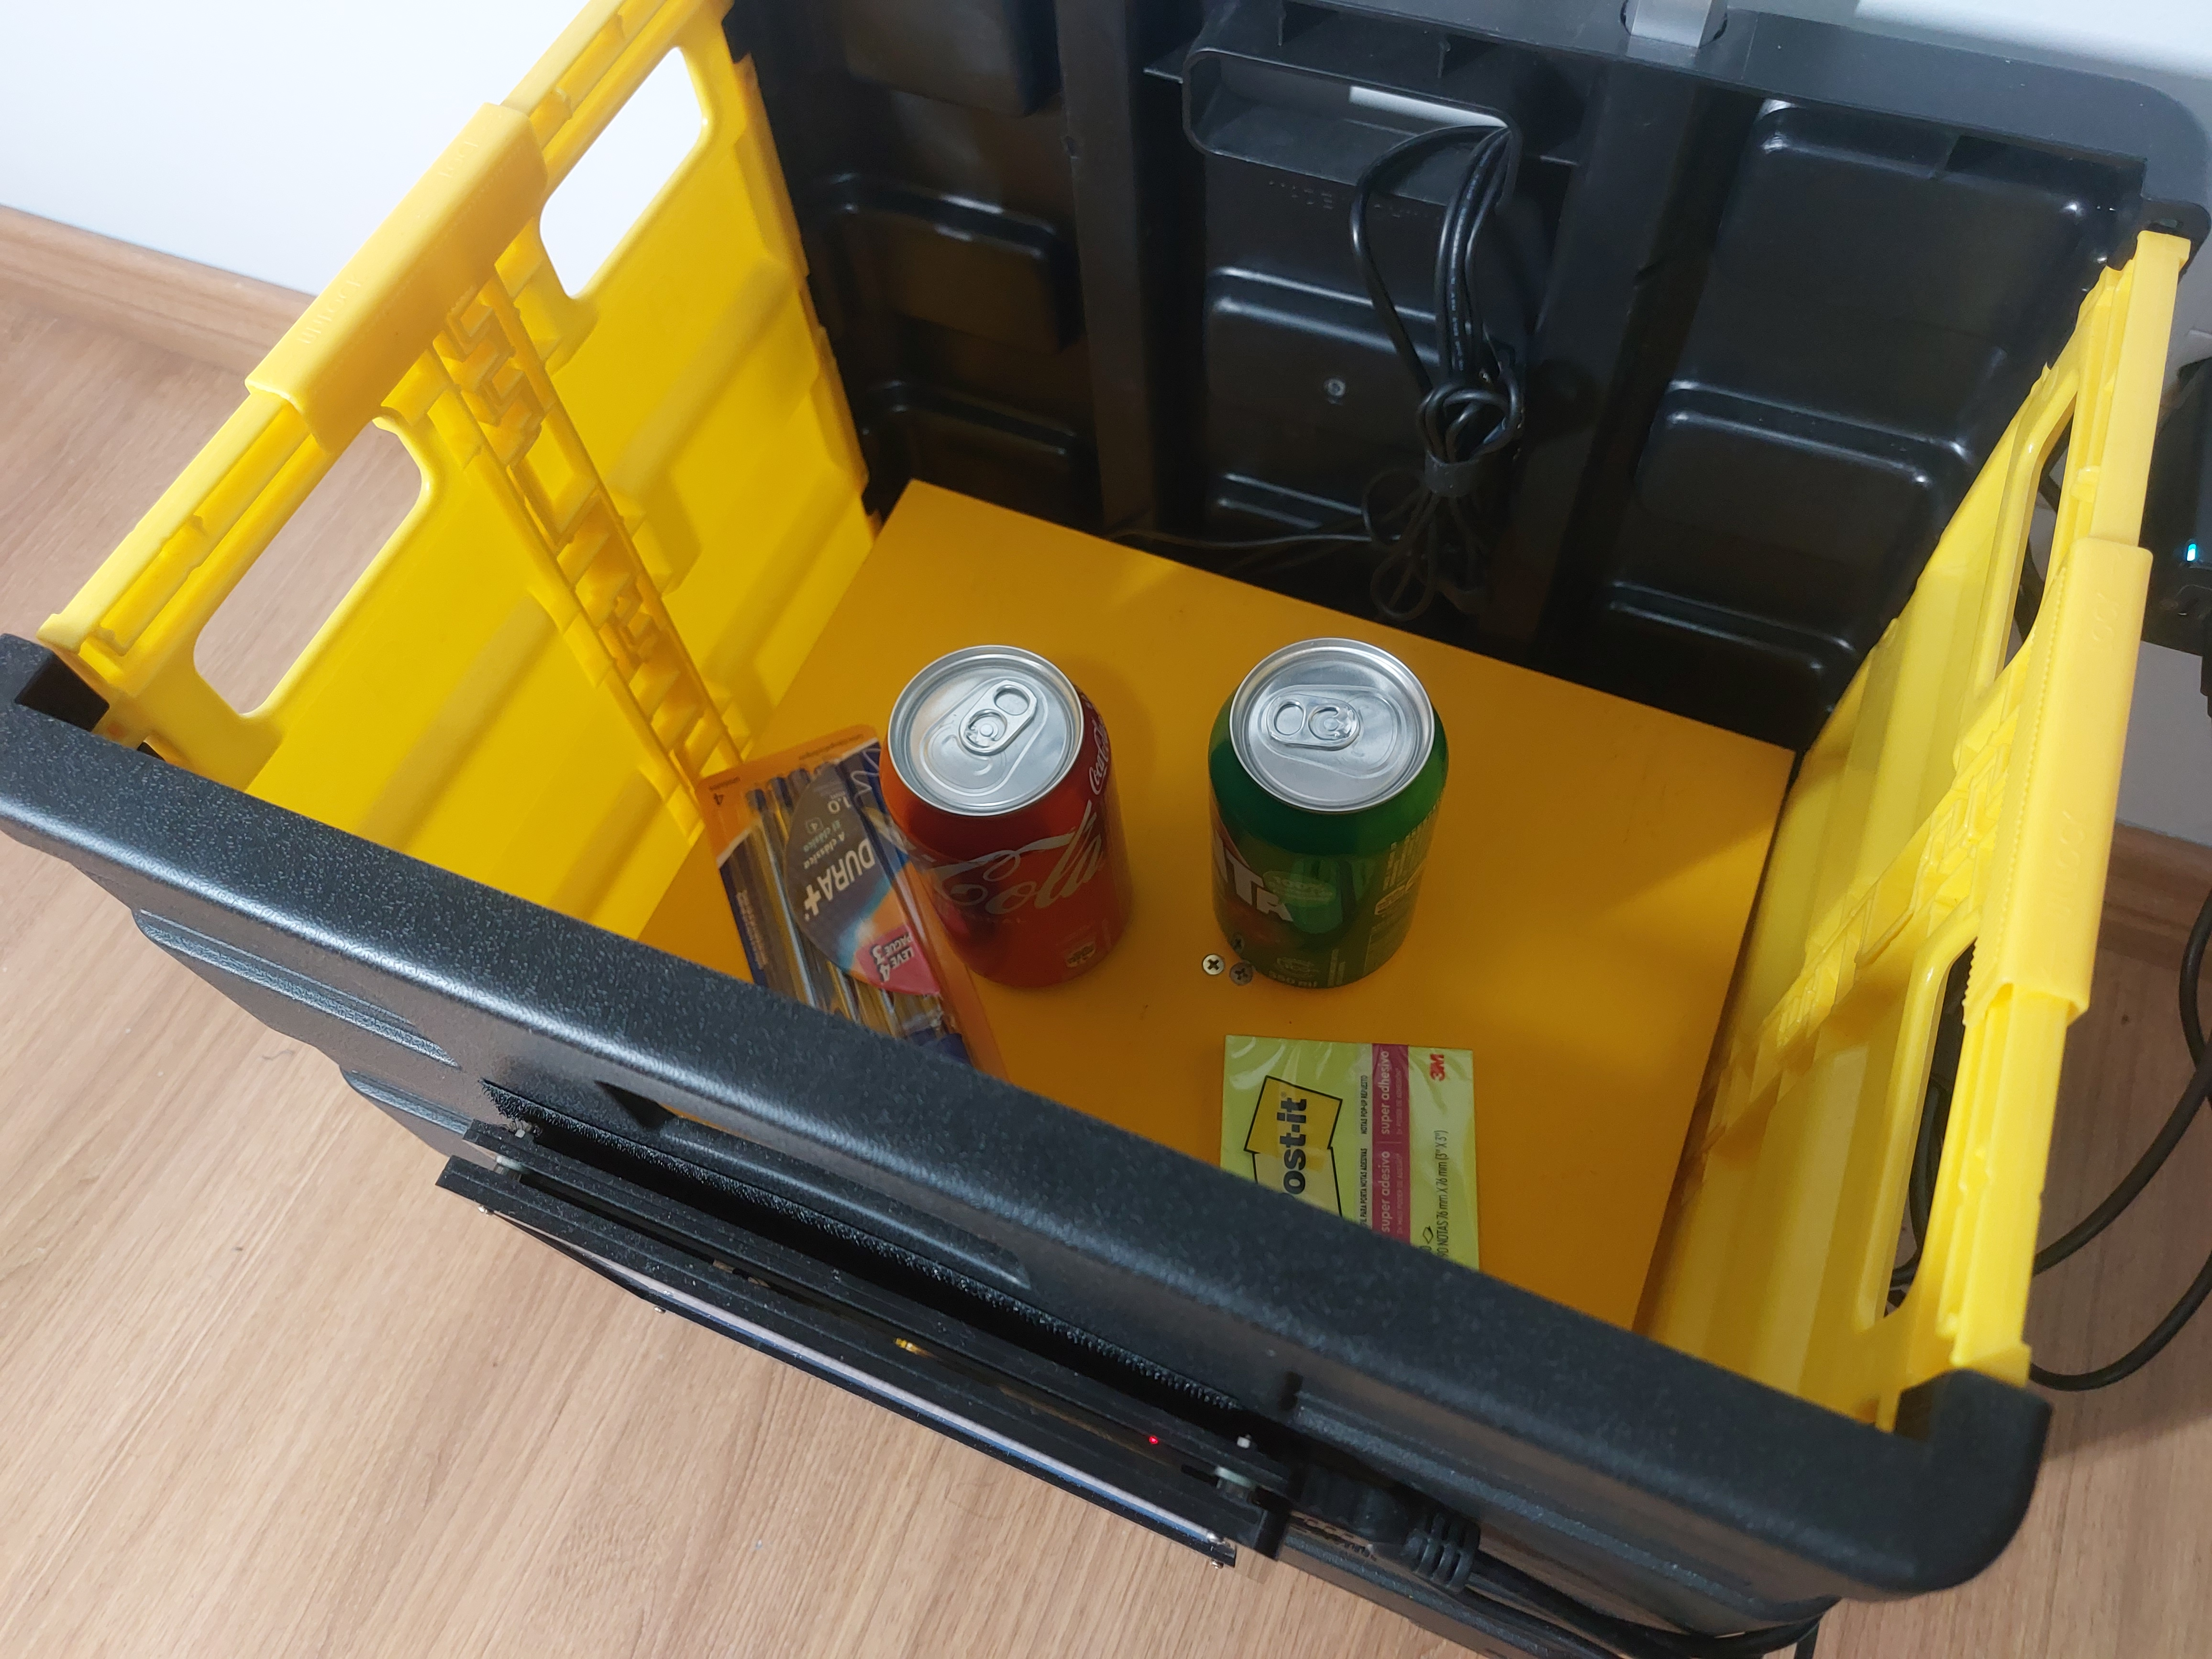
\includegraphics[width=0.8\textwidth]{./images/20221204_164147.jpg}
    \fonte{}
\end{figure}

\begin{figure}[H]
	\centering
	\caption[Frontal view of the prototype displaying the video camera feed]{Frontal view of the prototype displaying the video camera feed}
    \includegraphics[width=0.8\textwidth]{./images/20221204_163825.jpg}
    \fonte{}
\end{figure}

\begin{figure}[H]
	\centering
	\caption[Frontal view of the prototype displaying the video camera feed]{Frontal view of the prototype displaying the video camera feed}
    \includegraphics[width=0.8\textwidth]{./images/20221204_164136.jpg}
    \fonte{}
\end{figure}

\begin{figure}[H]
	\centering
    \caption[Popup confirmation before finishing the purchase]{Popup confirmation before finishing the purchase}
    \includegraphics[width=0.8\textwidth]{./images/20221204_161311.jpg}
    \fonte{}
\end{figure}

\begin{figure}[H]
	\centering
	\caption[Checkout confirmation screen]{Checkout confirmation screen}
    \includegraphics[width=0.8\textwidth]{./images/20221204_161314.jpg}
    \fonte{}
\end{figure}


\begin{figure}[H]
	\centering
	\caption[Product addition notification]{Product addition notification}
    \includegraphics[width=0.7\textwidth]{./images/20221204_164249.jpg}
    \fonte{}
\end{figure}

\begin{figure}[H]
	\centering
	\caption[Product removal notification]{Product removal notification}
    \includegraphics[width=0.7\textwidth]{./images/20221204_164237.jpg}
    \fonte{}
\end{figure}

